%%%%%%%%%%%%%%%%%%%%%%%%%%%%%%%%%%%%%%%%%%%%%%%%%%%%%%%%%%%%%%%%%%%%%%%%
%                                                                      %
%     File: Thesis_Bootrom.tex                        %
%     Tex Master: Thesis.tex                                %
%                                                                      %
%     Author: Carlos A. Rodrigues                         %
%     Last modified : 15 Abril 2013                         %
%                                                                      %
%%%%%%%%%%%%%%%%%%%%%%%%%%%%%%%%%%%%%%%%%%%%%%%%%%%%%%%%%%%%%%%%%%%%%%%

\chapter{Bootrom}
\label{chapter:Bootrom}

Quando um sistema arranca ou seja é dada energia ao sistema, este faz resite a todos os cores até mesmo ao processador. Depois do resite o processador vai ao endereço que é atribuido pela pessoas que desenvolver o sistema e carrega e carrega essa informação para o registo para começar a desenvolver o processo que está descrito a partir dessa posição de memoria. A partir daqui existe duas grande hipoteses, a primeira hipotese é o programa estar estar carregado na memoria de instruções partida. Tendo apenas o endereço de restart ser o endereço da memoria de instruções e ser o endereço onde começara o programa, este hipotese tem a vantagem de ser mais simples e de ter um restart mais rápido, começando o programa a correr assim que o sistema recebe energia, mas tem a desvantagem de o programa não poder ser alterado facilmente. a segunda Hipoetese é o endereço definido no restart ser um endereço para uma bootrom que tem disponível uma pequeno programa que copia o programa de uma memoria externa para a memoria de instruções, no fim de acabar esse processor coloca o o ponteiro do estrições para o endereço onde começa o programa que copiou de forma a executar o programa. esta segunda hipotese demora mais tempo o programa a iniciar, mas permite que o programa que se está a correr seja alteração de uma forma simples. Como por exemplo substituir um cartão de memoria e ligar e desligar a energia eléctrica do sistema. Uma bootrom é como o nome indica uma memoria Rom, apenas permite leitura, na maorias dos casos onde contem um pequeno programa normalmente escrito em assemble para ser mais pequeno e eficiente. Esse programa apenas copia os dados de uma determinado local para a memoria de instruções, podendo também fazer algumas pequenas verificações.

No desenvolvimento do projecto optou-se por utilizar uma bootrom por permitir uma alteração simples do programa que se estava a correr no sistema. A a comunidade openRisc tinha disponivel bastante simples que copiava os dados de HHHHH posições de memorias comeraçando de uma posição de endereços de periférico para outro endeço on estava localizado a sura memoria de enderços.
Mas era pretendido mais do que isso, para alem de copias essas posições de memoria pretendia-se que efectua-se verificações na correcta leitura da memoria onde o programa principal estava guardado e verificação de uma escrita correcta para a memoria de instruções. Para isso desenvolvemos uma bootroom que estão descrita no fluxograma \ref{fig:Fluxo_Bootrom} de uma forma sucinta.

escrever que isto é compilado e é possivel desactivar as cada mensagem de erro.

\begin{figure}[!htb]
  \centering
  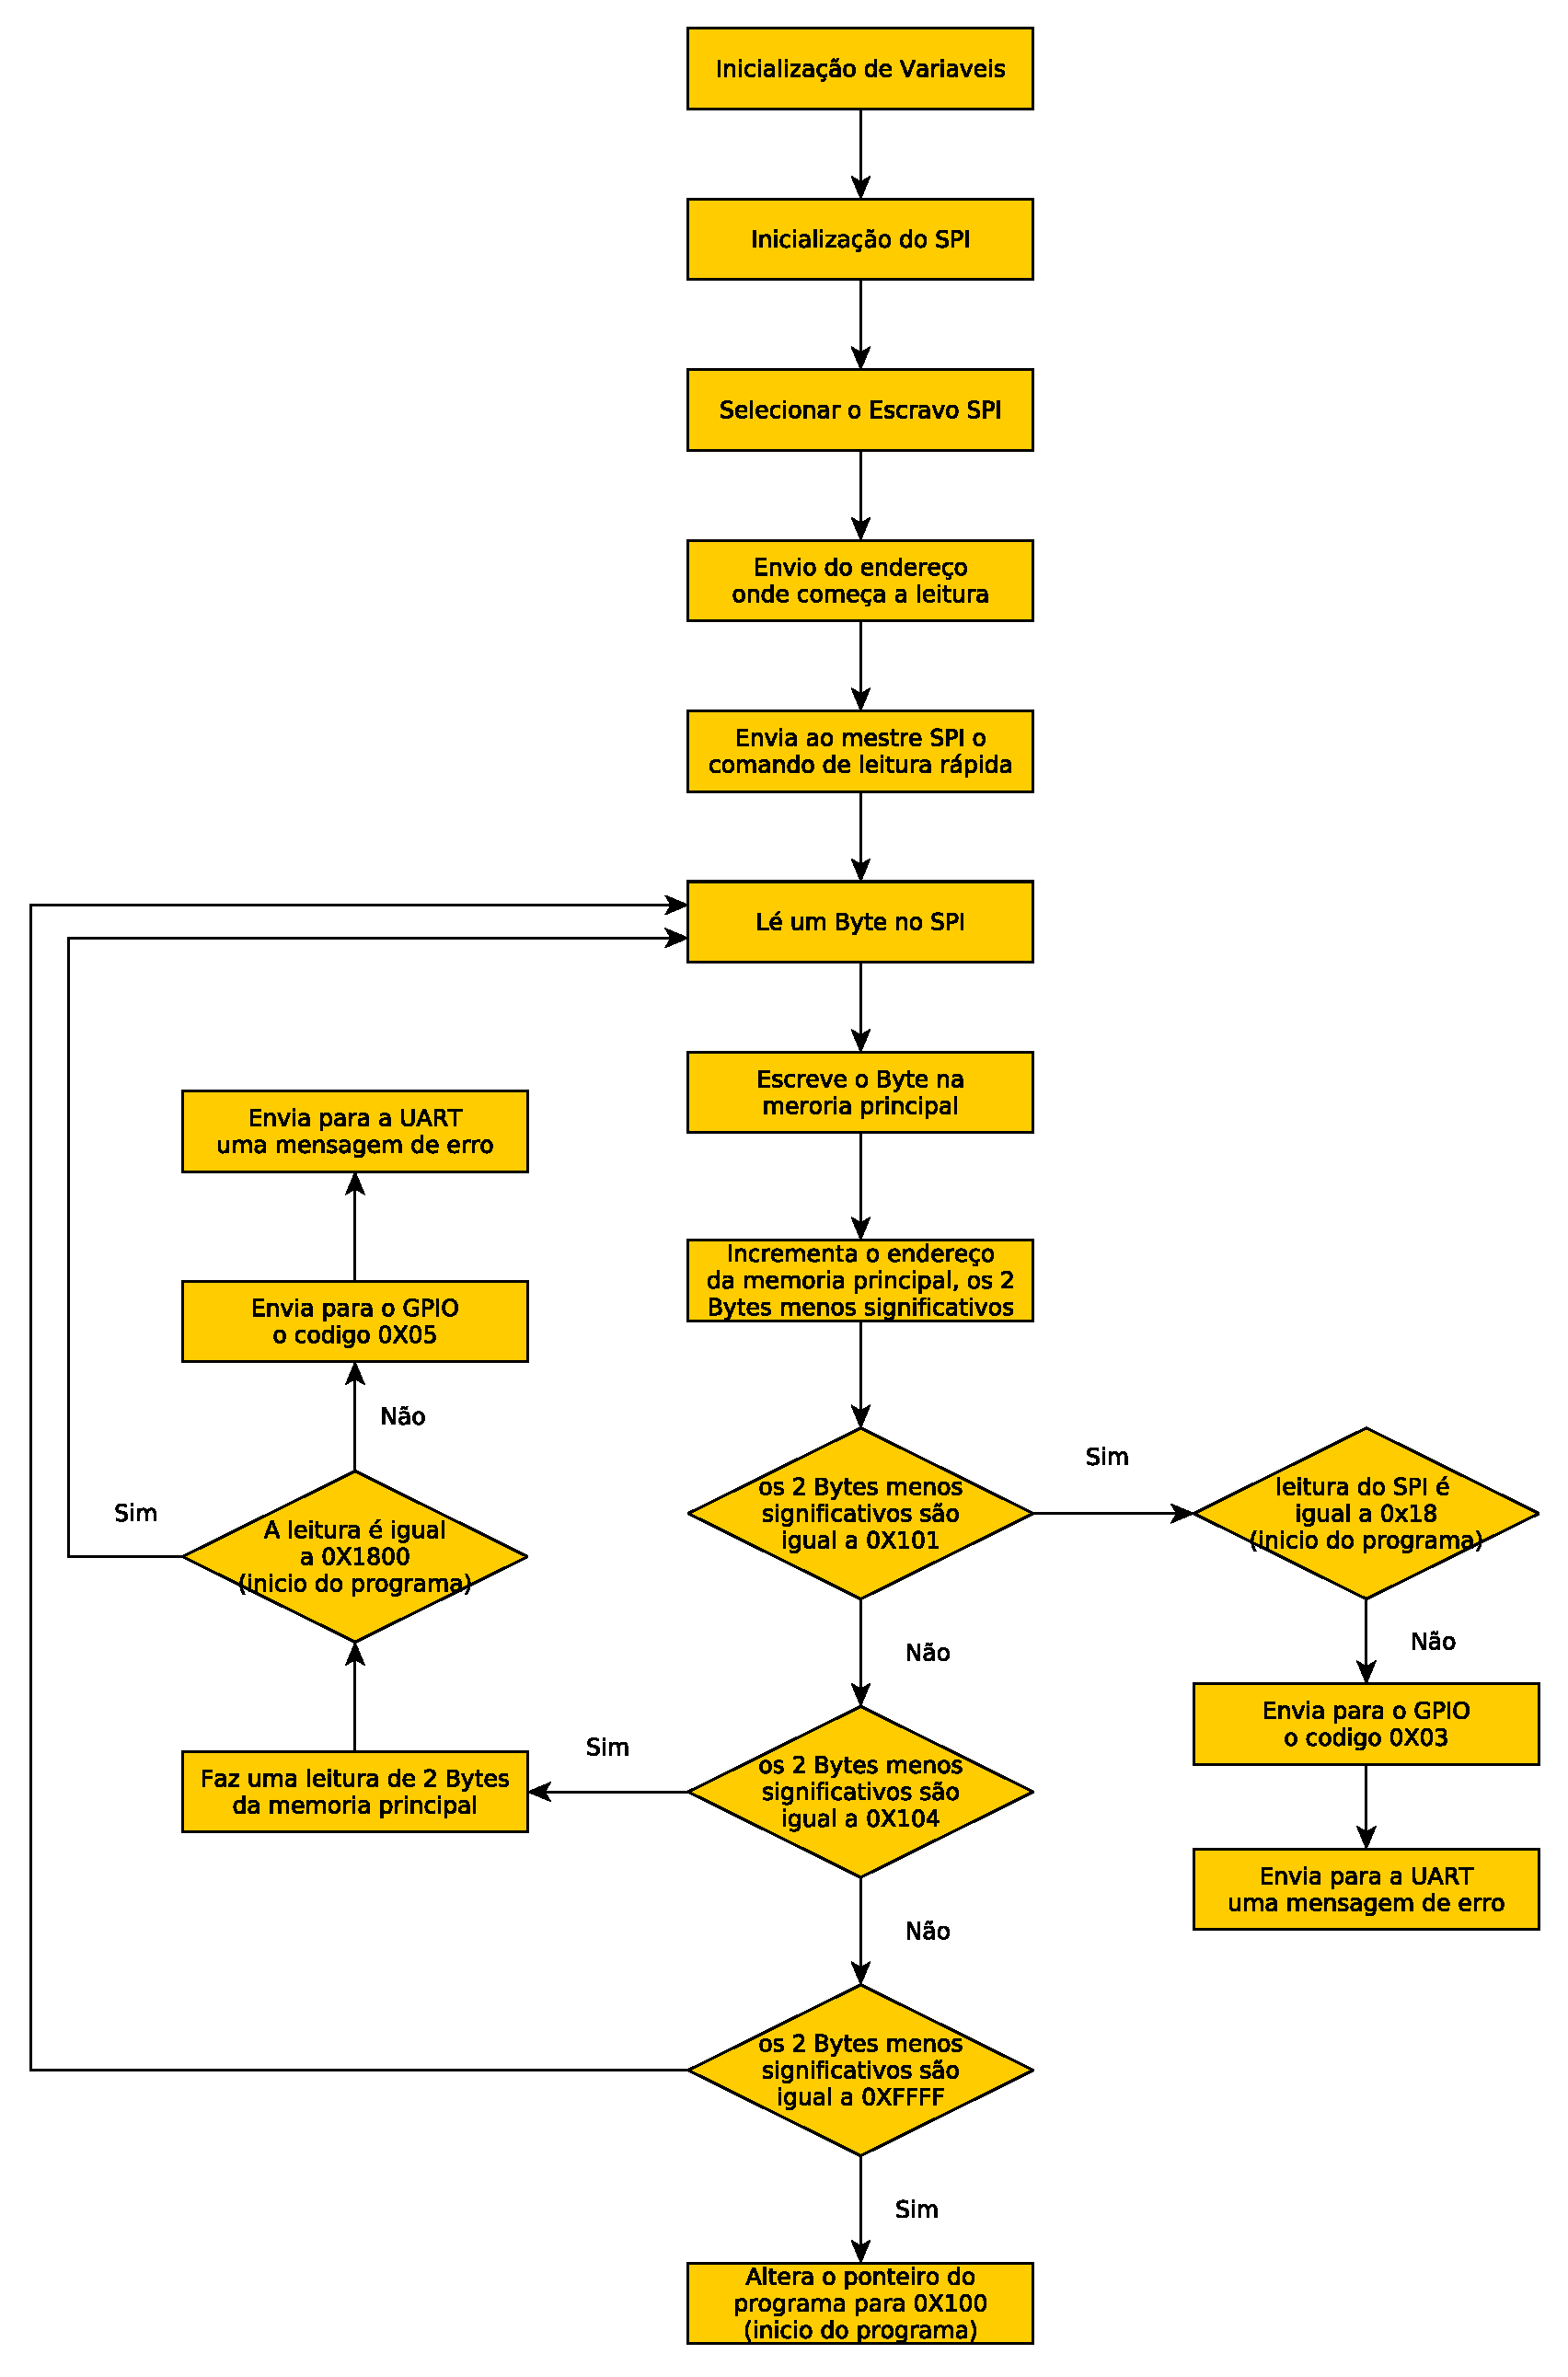
\includegraphics[width=0.75\textwidth]{grafos/Bootrom.pdf} %1  falta uma seta no fluxograma num exagno
  \caption[Fluxograma da Bootrom]{Fluxograma da Bootrom.}
  \label{fig:Fluxo_Bootrom}
\end{figure}

Como se pode ver pelo fluxograma a bootrom começa por iniciar os registo do processador, depois configura o core SPI. Inicializando o core mestre de SPI, informa o endereço que deve começar a ler da memroia e informar o tipo de leitura que pretende fazer neste caso a rápida. Começa a fazer uma leitura consegutiva de 0XFFFF(65535 na base decimal) posições de memoria, com palavras de tamanho de Byte. Quando acaba o envio de todas posições de memoria efetua uma salto do porteiro de instruções para a memoria de instruções para o endereço onde começa o programa, começando a correr o programa que estava na memoria externa. No ciclo que estão a efectuar a copia de uma memoria para outra, é efectuado dois testes para verificar que a correcta leitura e escrita das memorias. Quando é detectado um erro, este o core envia mensagens de erro tanto pela UART enviado uma mensagem de erro, e pela interface disponiblizada de GPIO envido um código de mensagem 0X03 se for problema de leitura da memoria externa e 0X05 se for problema de escrita na memoria interna.

\section{Testes de verifica\c{c}\~ao}
Os testes de verificação de leitura e escrita para verificar se foi correctamento um carregamento do programa na memomeria principal. Para isso foi desenvolvido um teste para cada caso de leitura dos dados da memoria externa que é lida por SPI e outro teste que verifica se foi escrito corretamente na memoria de instruções. 

\subsection{teste de leitura SPI}

O primeiro teste a ser efetuado é o teste de leitura das insctruções do programa da memoria externa por SPI. Todos os programas compilados têm a mesma instrução inicial 0X?????, na mesma posição de memoria 0X????. Neste teste ele everifica se os dados da posição de memoria 0X???? corresponden aos dados da instrução inicial. Como a memoria extrena tem apenas dois Bytes por cada posição o teste verifica os dois primeiro bytes da primeira instrução. Se os dados forem os esperados os ele continua a copias as instruções para a memoria de instruçoes se não, para de efectuar a copia dos instruções e enviar mensagens de erro tanto por GPIO como por UART. Quando detectado o processador envia um codigo de erro 0X?? para o GPIO e em seguida enviará a seguinte mensagem " mensagem XXX" pela UART. Caso tenha uma "leitor" de UART ligado ao sistema receberá a mensagem no meu leitor.

\subsection{teste de escrita na memoria principal }

O processo de teste é efectuado quando o processo de escrita para a memoria principal escreve os primeiros 4 Bytes de insctuções, correspondenedo ao endereço 0XWWWW da memoria principal. Quando a condição anterior é verdadeira a escrita de instruções é interrumpida momentaniamente, e é efectuado uma leitura de 4bytes do endereço  0XWWWW, que foi acabado de ser escrito. para verificar se as instruções estão a ser escritas correctamente a palavra lida na memoria principal tem de ser o valor 0XPPPPP, caso contrario existe algum erro no processo de escrita. Caso o teste seja positivo o processo continua normente a copiar as instruções do programa para a memoria principal, se não é dispuldado a seguinte mensagem de erro para a UART " mensagem de erro" do sistema e é colocado o seguinte codigo TT no GPIO.

explicar como é feito o teste de escrita na memoria principal 

como mostra o erro tanto com o GPIO como na uart.